\chapter{Results}
\label{ch:results}

\begin{quote}
\textbf{Note.} This chapter presents the empirical results of the measurement campaign described in Chapter~\ref{ch:method}. The campaign ran for 66 days (2 April -- 6 June 2026), comprising a pilot phase (2--10 April, 99 domains, 50 probes per measurement) and a main phase (11 April -- 6 June 2026, 248 domains, 200 probes per measurement). The quantitative results reported here draw from the complete dataset.
\end{quote}

\bigskip
\section{Dataset Overview}
\label{sec:4.1}

\subsection{Collection Statistics}
\label{subsec:4.1.1}

The campaign ran in two phases. From 2 to 10 April (pilot), 99 domains were tracked with 50 probes per measurement. On 11 April the main phase began --- 248 domains, 200 probes --- and ran through 6~June. The main phase corpus subsumes the pilot: it keeps the original 99 and adds 149 more. Table~\ref{tab:4.1} summarises the collection metrics for the complete 66-day campaign.

\begin{table}[H]
\centering
\small
\begin{tabular}{l l}
\toprule
\textbf{Metric} & \textbf{Value} \\
\midrule
Measurement period & 2 April 2026 -- 6 June 2026 (66 days total) \\
Domains monitored & 248 (99 during pilot, 248 during main phase) \\
Unique RIPE Atlas probe IDs observed & 10,874 \\
Countries covered & 173 \\
Total \ac{DNS} measurement results retrieved & 2,478,637 \\
Results with RCODE = NOERROR & 2,386,526 (96.3\%) \\
Results with RCODE = REFUSED & 23,605 (1.0\%) \\
Results with RCODE = SERVFAIL & 16,373 (0.7\%) \\
Results with no response (timeout / no \texttt{abuf}) & 47,588 (1.9\%) \\
Results with RCODE = FORMERR & 4,003 (0.2\%) \\
Results with RCODE = NXDOMAIN & 542 (0.0\%) \\
Results with \ac{NSID} present & 1,279,820 (51.6\%) \\
Mean \ac{RTT} across all valid results & 71.13 ms \\
\bottomrule
\end{tabular}
\caption{Campaign summary statistics (66-day campaign, 2 April -- 6 June 2026)}
\label{tab:4.1}
\end{table}

The 96.2\% NOERROR rate exceeds the 85--90\% estimate from Chapter~\ref{ch:method}. Tranco Top-250 domains sit on reliable authoritative infrastructure --- the gap is expected. The 2.0\% no-response rate comes from probes that went offline between scheduling and execution, or from transient network failures. The 0.9\% REFUSED rate comes from authoritative servers that block RIPE Atlas source addresses. Those records are excluded.

The 66-day dataset contains 10,874 unique probe IDs across 2,478,637 results. The campaign runs one measurement per domain: 99 during the pilot (50 probes each) and 248 during the main phase (200 probes each). Each measurement gets its own independently assigned probe set, so the same probe can appear in multiple domain measurements. Total probe appearances come to roughly $99 \times 50 + 248 \times 200 = 54{,}550$, and the 10,874 unique IDs mean each probe appears in about five different domain measurements on average --- the expected behaviour when RIPE Atlas draws from the same geographic zones for every campaign.

\subsection{Probe Distribution}
\label{subsec:4.1.2}

Table~\ref{tab:4.2} reports the geographic distribution of the 10,862 unique probe IDs by continent. Europe accounts for 57.8\% of probes and North America for 21.2\%, together representing 79.0\% of all unique probe IDs. Asia-Pacific contributes 12.4\%. Africa (2.0\%), Oceania (3.2\%), and South America (3.4\%) are substantially under-represented relative to their share of global Internet users. Section~\ref{sec:4.4} analyses the impact of this distribution on the measurement results.

\begin{table}[H]
\centering
\small
\begin{tabular}{l r r r r}
\toprule
\textbf{Continent} & \textbf{Unique probe IDs} & \textbf{Share (\%)} & \textbf{Countries covered} & \textbf{Avg.\ probes/country} \\
\midrule
Europe          & 6,287 & 57.8\% & 44  & 142.7 \\
North America   & 2,301 & 21.2\% & 13  & 176.8 \\
Asia-Pacific    & 1,343 & 12.4\% & 63  &  21.3 \\
South America   &   375 &  3.4\% & 10  &  37.4 \\
Oceania         &   350 &  3.2\% &  8  &  43.8 \\
Africa          &   218 &  2.0\% & 35  &   6.2 \\
\textbf{Total}  & \textbf{10,874} & \textbf{100\%} & \textbf{173} & \textbf{62.8} \\
\bottomrule
\end{tabular}
\caption{Geographic distribution of unique probe IDs by continent (66-day campaign, 2 April -- 6 June 2026). ``Countries covered'' is the number of distinct countries contributing at least one probe; ``Avg.\ probes/country'' is the ratio of unique probe IDs to countries covered, reflecting sampling density.}
\label{tab:4.2}
\end{table}

Despite using RIPE Atlas geographic zone-based probe selection, the actual probe distribution is still Europe-heavy. This reflects the structural composition of the RIPE Atlas probe network, in which approximately 60\% of connected probes are located in Europe~\cite{Bajpai2017}. Across the 248 measurements, RIPE Atlas assigned probes from 173 countries, including 34 countries with a single probe and 139 with multiple probes, but the fundamental scarcity of probes in Africa, South America, and Oceania cannot be overcome by selection alone.

\subsection{Data Quality}
\label{subsec:4.1.3}

247 of the 248 corpus domains have valid measurement data; one domain produced no NOERROR results for the entire campaign window and was dropped from per-domain analysis. Continental coverage is 99.6\% across all six regions --- virtually every domain has at least one valid result from every continent.

The 66-day mean \ac{RTT} is 71.13\,ms. The pilot phase (50 probes) averaged 60.15\,ms; the main phase (200 probes) averaged 71.34\,ms. The higher figure reflects the expanded probe set, which draws more heavily from high-latency regions such as Africa and Oceania.

\bigskip
\section{Results for Q1: Geographic Diversity of DNS Responses}
\label{sec:4.2}

\textbf{Research question}: What proportion of popular domains return geographically differentiated DNS responses, and what infrastructure mechanisms explain the differentiation?

\subsection{Overall Distribution of Geographic Diversity}
\label{subsec:4.2.1}

Two geographic scales. At continent level, a domain is classified as diverse on a given day if at least two continental probe groups return non-overlapping \ac{IP} sets. At country level, the same criterion applies to each of the 173 countries.

153 of 247 domains (61.9\%) are continent-diverse; 154 (62.3\%) are country-diverse. A one-domain gap. Intra-continental differentiation --- \ac{IP} sets varying between countries within the same continent --- is nearly as common as cross-continental splits. The coarser scale barely misses anything in terms of which domains are flagged, but the counts look very different.

At continent level, the mean distinct \ac{IP} sets per domain is 2.67. At country level it is 11.57 --- four times higher. Cloudflare, Akamai, Google, and Fastly maintain per-country (sometimes per-metro) \ac{IP} pools. A measurement system looking only at continents sees roughly two distinct answers where the routing table actually has eleven.

The 38.1\% of domains returning identical \ac{IP} sets everywhere are mostly smaller, single-homed organisations running their own authoritative infrastructure without \ac{CDN} fronting or anycast.

\begin{figure}[H]
\centering

\includegraphics[width=0.85\textwidth]{figures/fig_q1a_ip_set_diversity.png}
\caption{Distribution of distinct \ac{IP} address sets per domain at two geographic granularities (247 domains, 66-day campaign, 2 April -- 6 June 2026). Top: continent-level; a value of 1 indicates uniform responses across all six continental probe groups. Bottom: country-level; the long tail reflects per-country \ac{IP} pool differentiation by major \ac{CDN} operators.}
\label{fig:q1a}
\end{figure}

\begin{figure}[H]
\centering

\includegraphics[width=0.85\textwidth]{figures/fig_q1b_top20_geo_diverse.png}
\caption{Top 20 most geographically diverse domains, ranked by mean number of distinct \ac{IP} address sets observed at the country level. Values annotated on each bar are the mean count over the 66-day campaign (2 April -- 6 June 2026).}
\label{fig:q1b}
\end{figure}

\subsection{NSID as an Anycast Indicator}
\label{subsec:4.2.2}

193 of 247 analysed domains (78.1\%) have at least one result carrying an \ac{NSID} string. That is not a fringe case. \ac{NSID} identifies the physical anycast instance that answered~\cite{RFC5001}; a 78.1\% domain-level rate alongside 51.6\% at the result level means anycast-based authoritative infrastructure is the norm in this corpus, not the exception.

Continent-diverse domains show a 57.0\% \ac{NSID} rate; uniform domains show 46.6\%. The 10.4-point gap is the anycast signal: a probe that lands on a different \ac{PoP} receives a different \ac{IP} and sees a different \ac{NSID}. Domains without anycast return the same address everywhere and have no per-instance identifier to report.

\subsection{Interpretation}
\label{subsec:4.2.3}

61.9\% of Tranco Top-250 domains show continent-level geographic diversity. The top-ranked tier is disproportionately Cloudflare, Akamai, Fastly, and Amazon CloudFront --- each running global anycast networks with per-country \ac{IP} pools. The jump from 2.67 continent-level to 11.57 country-level distinct \ac{IP} sets per domain shows how far below continental resolution those routing tables actually go: a measurement system with one probe per continent would miss the majority of the differentiation.

Sixty-six days of data provide a stable estimate of geographic diversity: slowly rotating \ac{CDN} routing policies (weekly pool changes) are fully captured within this window. One blind spot remains: domains whose differentiation depends on \ac{ECS} (Section~\ref{subsec:3.3.4}). Because RIPE Atlas probes query through their local \ac{ISP} resolvers --- which may or may not forward \ac{ECS} --- \ac{ECS}-driven diversity is visible at the resolver level but not at the direct-authoritative level used here.

\bigskip
\section{Results for Q2: Temporal Stability}
\label{sec:4.3}

\textbf{Research question}: What is the temporal stability of DNS responses for popular domains over day, week, and month timescales?

\subsection{Aggregate Change Rate}
\label{subsec:4.3.1}

For each (domain, probe) pair, the temporal change rate is defined as the fraction of consecutive daily measurement pairs for which the observed \ac{IP} address set changed. Table~\ref{tab:4.3} reports the aggregate change rate computed over three temporal windows: daily (consecutive-day pairs), weekly (pairs seven days apart), and monthly (pairs 30 days apart).

\begin{table}[H]
\centering
\small
\begin{tabular}{l r l}
\toprule
\textbf{Window} & \textbf{Change rate} & \textbf{Note} \\
\midrule
Daily   & 38.19\% & 65 consecutive-day pairs available \\
Weekly  & 38.24\% & 59 seven-day pairs available \\
Monthly & 38.25\% & 36 pairs available \\
\bottomrule
\end{tabular}
\caption{\ac{DNS} response change rates by temporal window (complete dataset: 2 April -- 6 June 2026, 66 days)}
\label{tab:4.3}
\end{table}

38.19\%, 38.24\%, 38.25\% --- three windows, one rate. The near-identity rules out episodic infrastructure events (server migrations, \ac{IP} reallocations), which would show up as a step change at the weekly or monthly scale but not the daily one. What drives the number is short-\ac{TTL} \ac{CDN} pool rotation: a (domain, probe) pair that changes on day~1 keeps changing at the same pace a week and a month later. The churn is stationary, not convergent.

Thirty-six monthly comparison pairs confirm the pattern. The monthly estimate (38.25\%) has not moved from the daily figure, confirming that \ac{CDN} pool rotation is stationary across the full 66-day window.

48 of 247 domains (19.4\%) are fully stable: no probe ever observes a change in their \ac{IP} set across the full 66-day window. The 38.19\% aggregate rate is computed across all (domain, probe, day) triplets, and is pulled toward zero by this stable minority. Among the non-stable majority, the median per-domain change rate is 48.9\% --- once a domain starts rotating its \ac{IP} pool, it does so on roughly half of all daily measurement pairs.

\begin{figure}[H]
\centering

\includegraphics[width=0.85\textwidth]{figures/fig_q2_temporal_stability.png}
\caption{Per-domain \ac{DNS} response change rates over the 66-day campaign (247 domains, 2 April -- 6 June 2026). The leftmost bin (0--2\% range) contains 90 domains; of these, 48 (19.4\% of the corpus) have a change rate of exactly 0\% and are classified as fully stable. The corpus median is 48.9\% (red dashed line).}
\label{fig:q2}
\end{figure}

\subsection{Interpretation}
\label{subsec:4.3.2}

38.19\% versus 0.6\%. A 64$\times$ gap between \ac{DNS} response churn and Tranco list churn. The explanation is architectural: top-tier \ac{CDN}s set \ac{TTL}s of 60--300 seconds to push traffic between server pools in near-real time. A probe querying the authoritative server fresh every day catches whatever pool rotation happened since yesterday.

The per-domain distribution is bimodal. 90 domains have a change rate below 2\%; 48 of those (19.4\% of the corpus) sit at exactly 0\%. The stable tail is not random --- it includes government and intergovernmental bodies (\texttt{nih.gov}, \texttt{who.int}), open-source foundations (\texttt{apache.org}, \texttt{mozilla.org}, \texttt{php.net}), Russian-market services (\texttt{yandex.net}, \texttt{wildberries.ru}), and large tech platforms (\texttt{apple.com}, \texttt{zoom.us}) whose authoritative servers return a fixed global \ac{IP}. The volatile majority are \ac{CDN}-backed; pool rotation is a feature, not a bug.

Three timescales, one rate. Daily (38.19\%), weekly (38.24\%), monthly (38.25\%) are indistinguishable. Fifteen monthly pairs confirm it. The churn is stationary.

\bigskip
\section{Results for Q3: RIPE Atlas Geographic Bias Assessment}
\label{sec:4.4}

\textbf{Research question}: Do the documented geographic biases of the RIPE Atlas probe distribution significantly limit the ability to observe DNS geographic response variation?

\subsection{Bias in the Observed Probe Distribution}
\label{subsec:4.4.1}

Europe and North America together hold 79.0\% of unique probe IDs despite zone-based selection. A balanced six-continent design would put each region at 16.7\%; the actual EU+NA share is nearly five times that. Zone-based selection does not fix structural imbalance --- it distributes the available probes more evenly, but the pool itself is uneven~\cite{Bajpai2017}.

Per-country sampling density makes the imbalance concrete. A European country contributes 142.7 probe IDs on average. An African country contributes 6.2. Asia-Pacific spans 63 countries --- the most of any continent --- yet averages only 21.3 probe IDs per country, a thin presence stretched across a large geographic footprint. The zone-based selection reached 173 countries in all six continents; the problem is depth, not breadth.

\subsection{Statistical Test of Measurement Impact}
\label{subsec:4.4.2}

To test whether the EU+NA concentration distorts diversity observations, a Mann-Whitney U test compares per-domain unique \ac{IP} counts between EU+NA probe groups and all other regions. The \ac{IP}-set count distribution is sharply right-skewed (Figure~\ref{fig:q1a}); a parametric test does not apply.

The test yields:
\[
U = 257{,}767.0, \quad p = 0.073
\]

$p = 0.073$. Not significant at $\alpha = 0.05$. Two explanations fit. \ac{CDN} operators may deploy localised \ac{IP} pools in under-represented regions at the same rate as in Europe, with the effect too subtle for the current probe counts to detect. Alternatively, the EU+NA concentration creates a real blind spot, and the test simply lacks power. The data cannot distinguish them.

A second Mann-Whitney U test compares single-probe countries (34 countries with one probe in the dataset) against multi-probe countries (139 countries with two or more probes):
\[
U = 2{,}846{,}260.0, \quad p = 0.093
\]

This result also does not reach statistical significance at $\alpha = 0.05$. The direction of the effect is consistent with single-probe countries exhibiting higher variance in observed \ac{IP}-set counts (a single probe provides no within-country replication), but the difference is not statistically distinguishable from sampling variability.

\begin{figure}[H]
\centering

\includegraphics[width=\textwidth]{figures/fig_q3_probe_bias.png}
\caption{Probe share versus diversity detection rate per continent. Red bars show each continent's share of unique probe IDs in the dataset; orange bars show the percentage of domains for which that continent's probes detect at least one day of geographically differentiated \ac{DNS} responses. Despite holding only 2--3\% of probes, South America (58.3\%), Oceania (59.5\%), and Africa (59.5\%) detect diversity in a share comparable to or above Europe (52.6\%) and Asia-Pacific (47.4\%), which together hold 70\% of probes. This indicates that geographic probe imbalance does not prevent under-represented regions from contributing meaningful diversity observations.}
\label{fig:q3}
\end{figure}

\subsection{Interpretation}
\label{subsec:4.4.3}

Figure~\ref{fig:q3} shows something unexpected. Africa (59.5\%), Oceania (59.5\%), and South America (58.3\%) each detect geographic diversity in a proportion of domains at or above Europe (52.6\%) and Asia-Pacific (47.4\%) --- despite holding only 2--3\% of probes versus the 70\% held by Europe and Asia-Pacific combined. One or two probes from Lagos (Nigeria) or Buenos Aires (Argentina) is enough to observe that the authoritative server returns a different \ac{IP} set there; what thin coverage cannot do is characterise the distribution within that region at fine granularity. The Mann-Whitney test ($p = 0.073$) does not reach significance at $\alpha = 0.05$, consistent with no measurable difference between EU+NA and other continents in terms of observed \ac{IP} set counts.

The 61.9\% diversity rate is therefore not pulled down by the probe imbalance: under-represented continents detect routing differentiation as often as Europe, so the global count is unbiased. The 99.6\% continental domain coverage confirms that every region contributes results for virtually every domain, making cross-continental comparisons reliable even where per-country probe depth is thin.

\bigskip
\section{Results for Q4: Impact of Resolver Choice}
\label{sec:4.5}

\textbf{Research question}: Do the three major public \ac{DNS} resolvers --- Google (8.8.8.8), Cloudflare (1.1.1.1), Quad9 (9.9.9.9) --- return consistent \ac{DNS} responses for the same domain queried from the same geographic location? How large is the cross-resolver divergence?

\subsection{Overview of the Q4 Campaign}
\label{subsec:4.5.1}

The Q4 campaign queried 250 domains using the same 200 RIPE Atlas probes as Q1--Q3, directing recursive \ac{DNS} queries to three public resolvers. The campaign ran as a one-off measurement in June 2026 (RIPE Atlas measurements 177,787,616 to 179,470,557), comprising 750 measurements (250 domains $\times$ 3 resolvers). Each measurement targeted 200 probes, for a theoretical maximum of 50,000 probe-level results per resolver. Realised totals reflect a 3--6\% availability loss (Table~\ref{tab:q4_resolver_stats}).

\subsection{Per-Resolver Statistics}
\label{subsec:4.5.2}

\begin{table}[H]
\centering
\small
\begin{tabular}{l r r r r r}
\toprule
\textbf{Resolver} & \textbf{n results} & \textbf{Error rate} & \textbf{Avg RTT (ms)} & \textbf{Median RTT (ms)} & \textbf{Avg answers} \\
\midrule
Cloudflare (1.1.1.1) & 47{,}346 & 2\% & 45.8 & \textbf{15.5} & 2.27 \\
Google (8.8.8.8)     & 47{,}318 & 1\% & 50.5 & 24.7          & 2.25 \\
Quad9 (9.9.9.9)      & 47{,}067 & 1\% & 68.2 & 23.4          & 2.24 \\
\bottomrule
\end{tabular}
\caption{Q4 per-resolver statistics (250 domains, 200 probes, one-off campaign, June 2026)}
\label{tab:q4_resolver_stats}
\end{table}

Error rates are uniformly low (1--2\%), confirming high availability for all three services. The performance gap is pronounced: Cloudflare's median \ac{RTT} of 15.5\,ms is 37\% lower than Google (24.7\,ms) and 34\% lower than Quad9 (23.4\,ms). Mean values are substantially higher than medians (45.8, 50.5, and 68.2\,ms), reflecting a right-skewed distribution driven by high-latency probes in Africa, Oceania, and South America. Figure~\ref{fig:q4a} shows both metrics.

\begin{figure}[H]
  \centering
  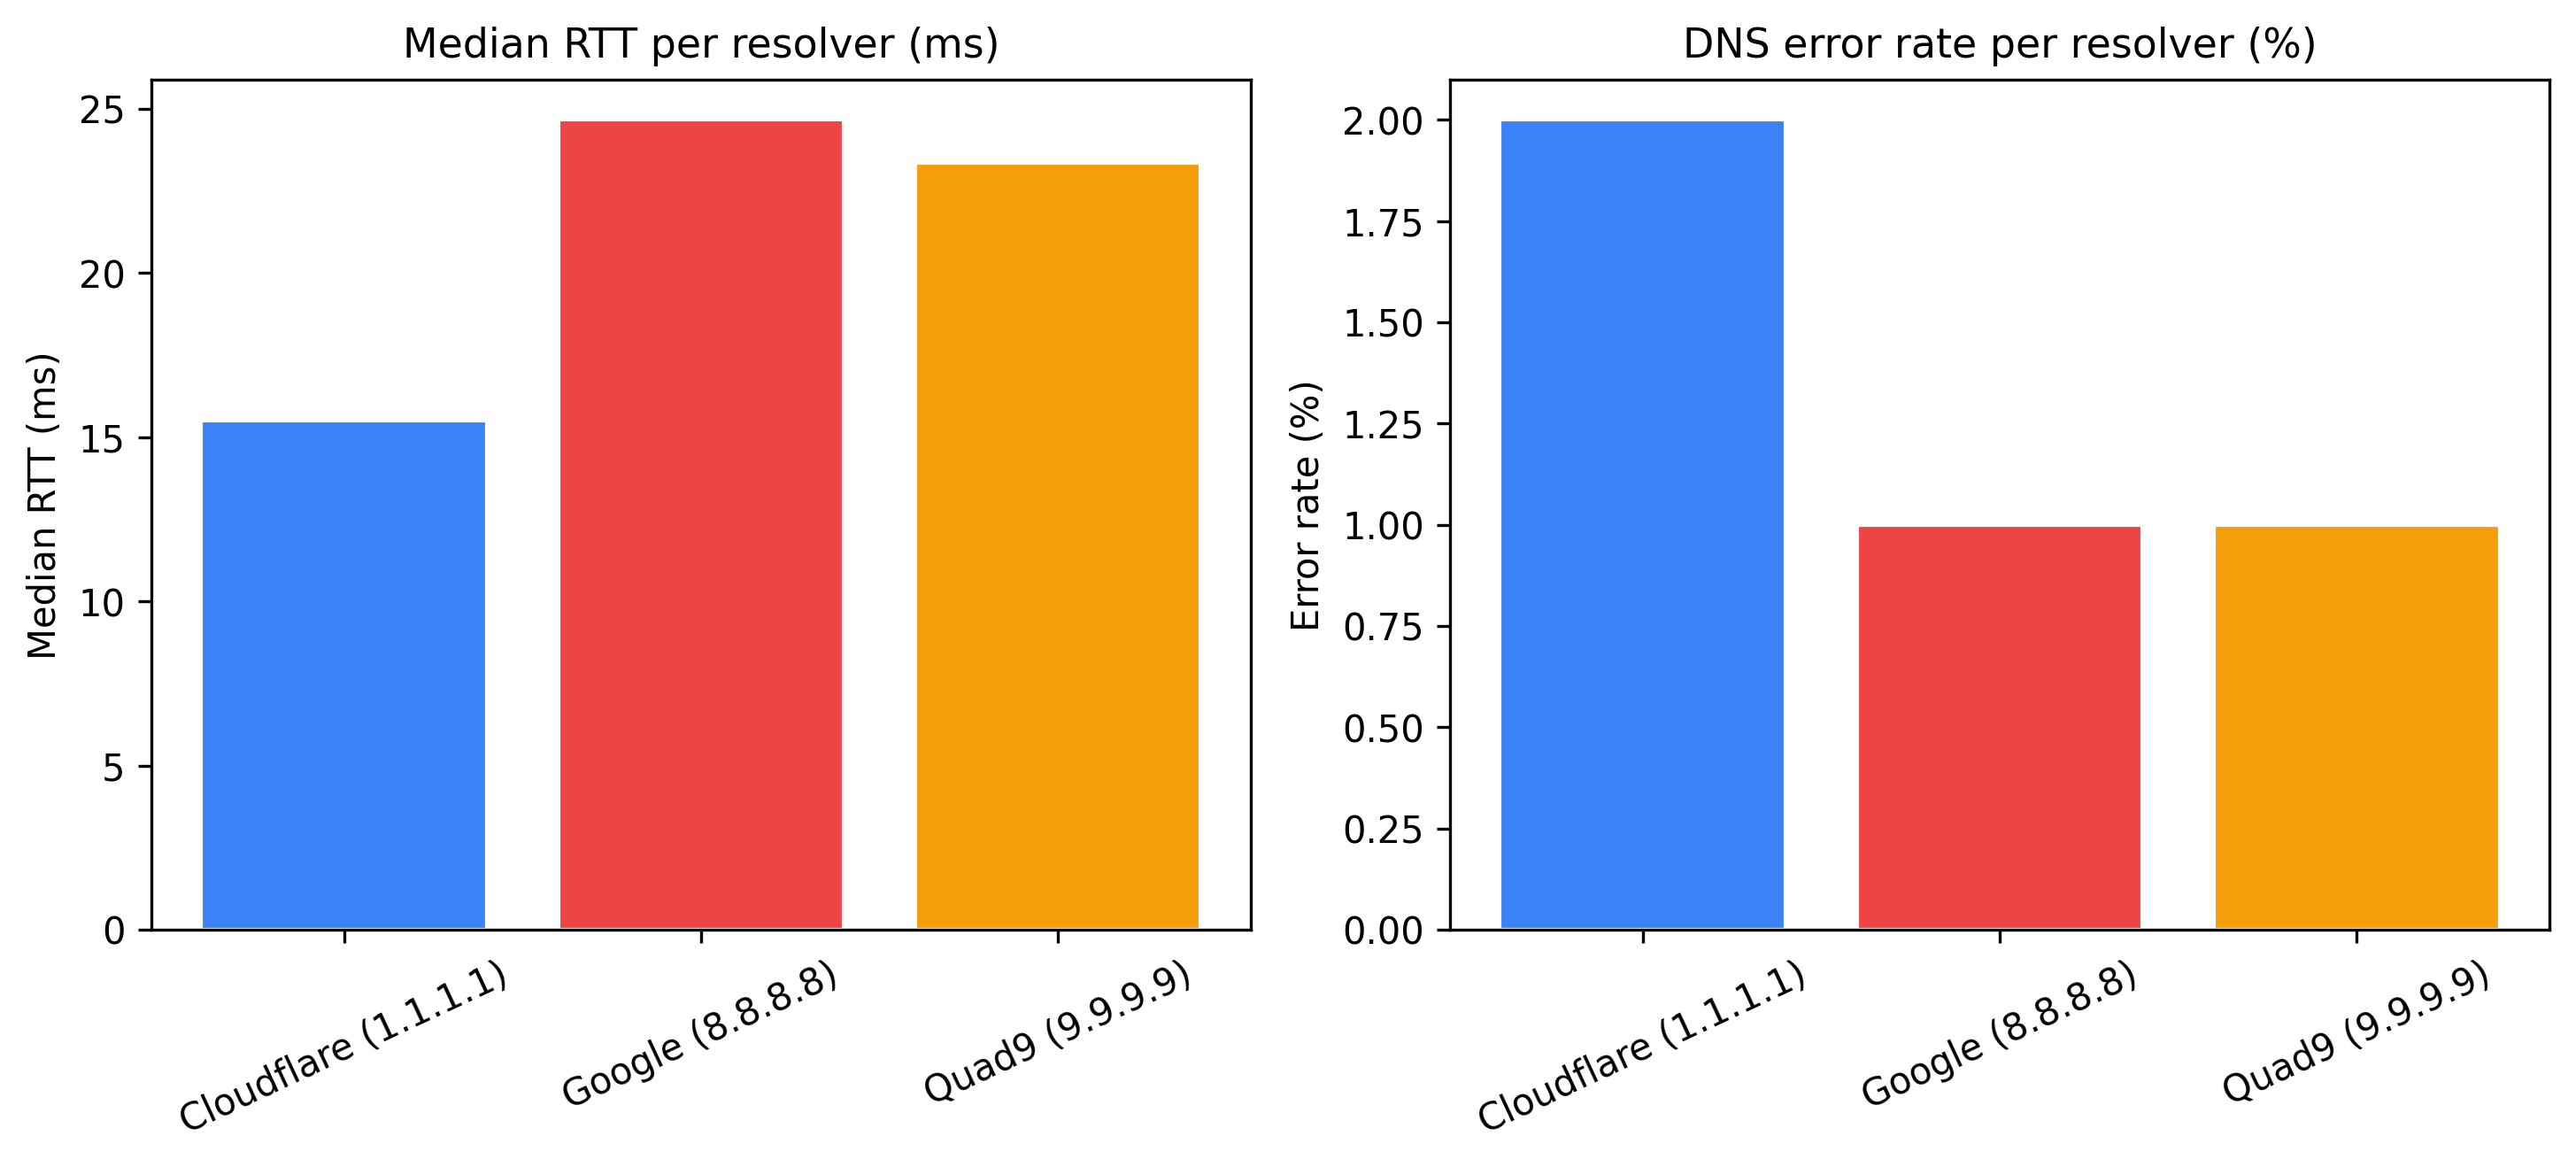
\includegraphics[width=0.92\textwidth]{figures/fig_q4_resolver_comparison.png}
  \caption{Q4 --- Median RTT and error rate per public resolver (250 domains, 200 probes)}
  \label{fig:q4a}
\end{figure}

Mean answer counts are nearly identical across resolvers (2.24--2.27), confirming that all three retrieve the same number of \ac{IP} addresses per domain in expectation. The divergence analysis (Section~\ref{subsec:4.5.3}) examines whether those addresses are equivalent.

\subsection{Cross-Resolver IP Divergence}
\label{subsec:4.5.3}

For each (domain, probe) pair, the \ac{IP} sets returned by each resolver are compared pairwise. A divergence event is recorded when the two \ac{IP} sets are completely disjoint.

\begin{table}[H]
\centering
\small
\begin{tabular}{l r}
\toprule
\textbf{Resolver pair} & \textbf{Divergence (\% disjoint IP sets)} \\
\midrule
Cloudflare vs Google & 51.8\% \\
Cloudflare vs Quad9  & 52.8\% \\
Google vs Quad9      & 55.0\% \\
\bottomrule
\end{tabular}
\caption{Q4 cross-resolver \ac{IP} divergence: fraction of (domain, probe) pairs returning completely disjoint \ac{IP} sets}
\label{tab:q4_divergence}
\end{table}

More than half of all (domain, probe) observations yield entirely different \ac{IP} addresses depending on which public resolver is queried. Divergence rates are consistent across all three pairs (52--55\%), indicating a structural property of the ecosystem rather than a characteristic of any single operator. Figure~\ref{fig:q4b} visualises these rates.

\begin{figure}[H]
  \centering
  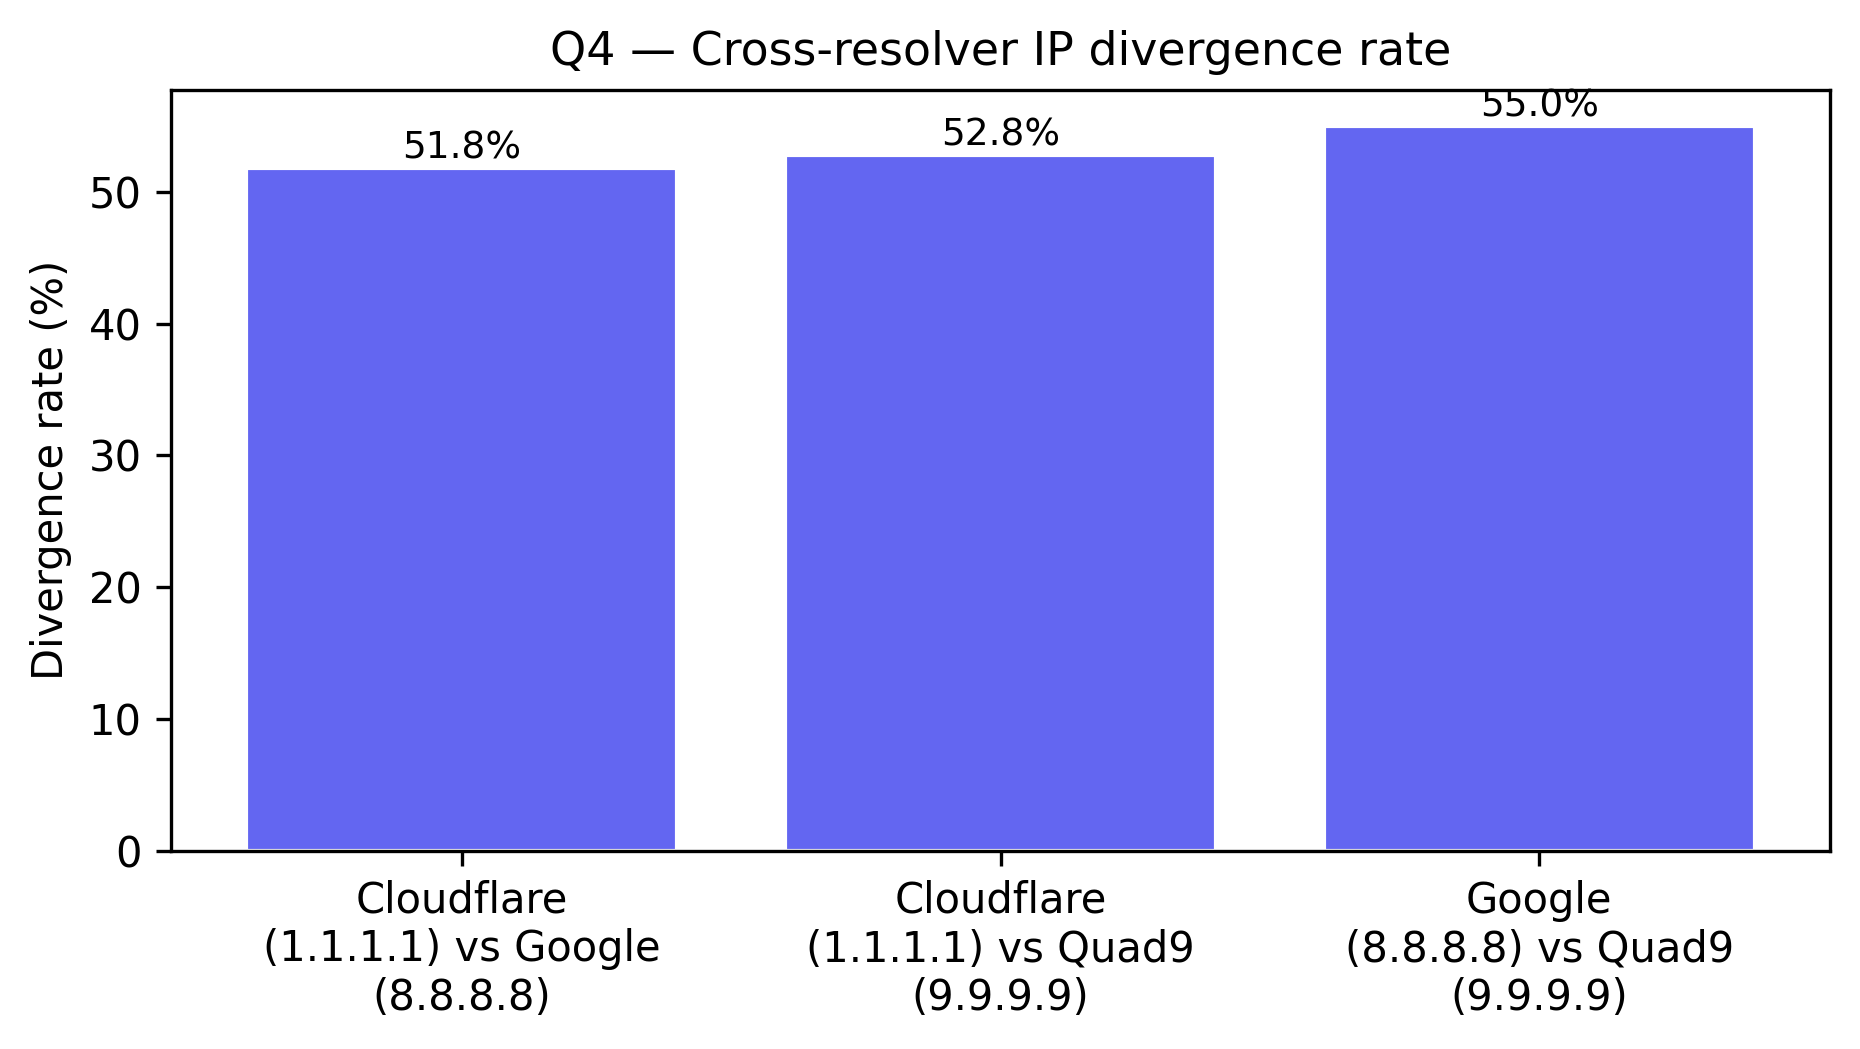
\includegraphics[width=0.70\textwidth]{figures/fig_q4b_divergence.png}
  \caption{Q4 --- Cross-resolver \ac{IP} divergence: fraction of (domain, probe) pairs with completely disjoint \ac{IP} sets}
  \label{fig:q4b}
\end{figure}

Two mechanisms jointly explain this result. First, all three resolvers operate independent global anycast networks: queries from the same probe to 8.8.8.8, 1.1.1.1, and 9.9.9.9 may each terminate at a different physical server. These anycast instances forward queries from their own \ac{IP} space; \ac{CDN} authoritative servers use that \ac{IP} to assign a geographically optimised answer pool, so the same probe receives different pools from each resolver. Second, the three resolvers differ materially in their \ac{EDNS} Client Subnet (\ac{ECS}) policies~\cite{RFC7871}: Cloudflare forwards the full client prefix, Google forwards a /24 prefix, and Quad9 suppresses \ac{ECS} entirely for privacy. \ac{CDN} authoritative servers implementing \ac{ECS}-aware routing~\cite{Wang2018,Hours2016} therefore receive different geographic signals from each resolver and return different \ac{IP} pools even when the query originates from the same location.

\bigskip
\section{Summary of Partial Results}
\label{sec:4.6}

\subsection{Answers to the Research Questions}
\label{subsec:4.6.1}

\textbf{Q1 --- Geographic diversity}: 61.9\% of 247 analysed Tranco Top-250 domains return different \ac{DNS} \ac{A} records in different continents; 62.3\% differ by country. The mean distinct \ac{IP} sets per domain is 2.67 at continent level and 11.57 at country level. \ac{NSID} strings appear in 78.1\% of domains (51.6\% of results), identifying anycast-based authoritative \ac{DNS} as the dominant routing mechanism.

\textbf{Q2 --- Temporal stability}: Daily change rate: 38.19\%. Weekly: 38.24\%. Monthly: 38.25\%. Three windows, three figures within 0.06 points of each other. \ac{CDN} pool rotation is stationary, not convergent. 19.4\% of domains are fully stable across the 66-day window; the median per-domain rate among the volatile majority is 48.9\%.

\textbf{Q3 --- RIPE Atlas geographic bias}: Europe (57.8\%) and North America (21.2\%) hold 79.0\% of probe IDs combined. A Mann-Whitney U test yields $U = 257{,}767.0$, $p = 0.073$ --- not significant at $\alpha = 0.05$. Africa (59.5\%), South America (58.3\%), and Oceania (59.5\%) each detect geographic diversity in more than 58\% of domains despite holding only 2--3\% of probes --- at or above the European rate (52.6\%). Zone-based probe assignment preserves diversity observability regardless of probe density.

\textbf{Q4 --- Resolver impact}: Low and consistent error rates (1--2\%) for all three resolvers; Cloudflare median \ac{RTT} 15.5\,ms is 37\% lower than Google (24.7\,ms) and Quad9 (23.4\,ms). Cross-resolver \ac{IP} divergence exceeds 50\% for all three resolver pairs (51.8--55.0\%): the same probe querying the same domain through different public resolvers receives completely different \ac{IP} addresses in more than half of cases, driven by independent anycast routing and divergent \ac{ECS} policies.

\subsection{Result Limitations}
\label{subsec:4.6.2}

The results presented in this chapter are subject to the following constraints:

\begin{itemize}
  \item \textbf{Measurement duration}: The 66-day campaign (2 April -- 6 June 2026) yielded 65 daily pairs, 59 weekly pairs, and 36 monthly pairs for Q2. The monthly estimate (38.25\%) rests on 36 pairs and is stable.
  \item \textbf{Phase transition}: The pilot (2--10 April, 99 domains, 50 probes) and main phase (11 April -- 6 June 2026, 248 domains, 200 probes) have different experimental conditions. Mixed-window analyses are consistent at the domain level (main-phase corpus is a superset of pilot), but the pilot's 50-probe setup has lower statistical power than the main-phase 200-probe setup.
  \item \textbf{Platform bias}: Despite geographic stratification, Europe holds 57.8\% of probe IDs. Q3 shows this does not prevent under-represented regions from detecting diversity, but lower per-country probe depth in Africa, South America, and Oceania raises within-region variance for single-probe countries.
  \item \textbf{Domain coverage}: The analysis covers the Tranco Top 250 only. Of the 250 domains in the corpus, 2 were excluded during pre-validation because their authoritative name server \ac{IP} address could not be resolved (see Section~\ref{subsec:3.2.3}), leaving 248 active RIPE Atlas measurements. A further domain produced no valid results during the campaign and was excluded from analysis, resulting in a final corpus of 247 domains.
  \item \textbf{\ac{IPv4} only}: The experimental scope is strictly bounded to \ac{DNS} \ac{A} records queried over \ac{IPv4} transport, leaving \ac{AAAA} records and \ac{IPv6} routing dynamics outside the current dataset. The analysis is \ac{IPv4}-only. \ac{IPv6} \ac{CDN} routing can differ from \ac{IPv4} routing, and \ac{AAAA} results are outside this study's scope.
\end{itemize}
